\subtop{Grundbegriffe}
%\newcounter{temp}
\vspace*{-0.5\baselineskip}\begin{description}
	\item[konvexe Kombination (von  $p_1,p_2$):] irgendein Punkt zwischen den beiden Punkten $p_1$ und $p_2$ oder auch $p = (1-\alpha)\cdot p_1 + \alpha\cdot p_2$ wobei $\alpha$ den Abstand zum Punkt $p_1$ beschreibt
	\item[(Linien-)Segment (mit den Endpunkten $p_1,p_2$):] die Menge $\overline{p_1p_2}= \{(1-\alpha)\cdot p_1 + \alpha\cdot p_2; 0\leq \alpha\leq 1\}$ aller konvexen Kombinationen von $p_1,p_2$
	\item[gerichtetes (Linien)-Segment (von $p_1$ nach $p_2$):] (Linien-)Segment definiert durch die Abbildung\\ $\overrightarrow{p_1p_2} : [0,1] \longrightarrow \mathbb{R}$ mit $\alpha \mapsto (1-\alpha)\cdot p_1 + \alpha\cdot p_2$
\end{description}

\subsection{Probleme}
\begin{enumerate}
	\item liegt $\overrightarrow{p_0p_1}$ rechts von $\overrightarrow{p_0p_2}$: \\
		\resizebox{1.5cm}{!}{\usetikzlibrary{arrows}

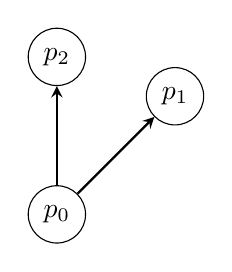
\begin{tikzpicture}[every node/.style={draw,circle}]

\node (0) at (0,0) {$p_0$};
\node (1) at (1.5,1.5) {$p_1$};
\node (2) at (0,2) {$p_2$};

\draw[->,>=stealth,thick](0)--(1);
\draw[->,>=stealth,thick](0)--(2);

\end{tikzpicture}}
	\item muss man auf dem von $p_0$ nach $p_2$ rechts abbiegen:\\
		\resizebox{!}{1.5cm}{\usetikzlibrary{arrows}

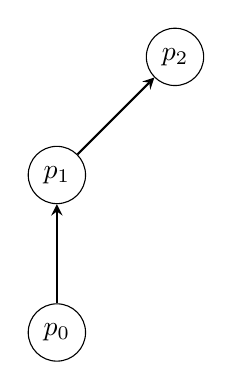
\begin{tikzpicture}[every node/.style={draw,circle}]

\node (0) at (0,0) {$p_0$};
\node (1) at (0,2) {$p_1$};
\node (2) at (1.5,3.5) {$p_2$};

\draw[->,>=stealth,thick](0)--(1);
\draw[->,>=stealth,thick](1)--(2);

\end{tikzpicture}}
	\item schneiden sich die beiden Liniensegmente $\overline{p_1p_2}$ und $\overline{p_3p_4}$:\\
		\resizebox{1.5cm}{!}{\usetikzlibrary{arrows}

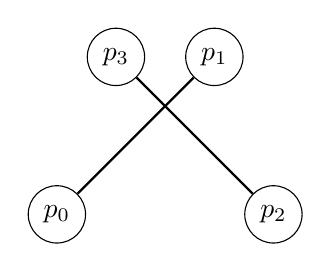
\begin{tikzpicture}[every node/.style={draw,circle}]

\node (0) at (0,0) {$p_0$};
\node (1) at (2,2) {$p_1$};
\node (2) at (2.75,0) {$p_2$};
\node (3) at (.75,2) {$p_3$};

\draw[thick](0)--(1);
\draw[thick](2)--(3);

\end{tikzpicture}}
\end{enumerate}

\subsection*{Lösungsansätze}
\begin{enumerate}
	\item Problem:
		\begin{itemize}
			\item bei der Transformation $p \mapsto p-p_0$ nehmen wir an, dass $p=(0,0)$ der Ausgangspunkt ist
			\item wir nehmen an, dass $x_1,x_2,y_1,y_2 \geq 0$
			\item wir nehmen an, dass $\overrightarrow{p_0p_1}$ rechts von $\overrightarrow{p_0p_2}$ liegt
			\item auf dem folgenden Parallelogramm ist $(t,0)$ der Schnittpunkt der x-Achse und der Linie durch $p_1$ sowie $p_1+p_2$:\\
				\begin{minipage}{0.3\textwidth}
					\usetikzlibrary{arrows,positioning,patterns}
\usetikzlibrary{shapes.geometric}
\usetikzlibrary{decorations.pathreplacing}

\begin{tikzpicture}[]
\coordinate (y2) at (0,2);
\coordinate (c) at (1,2);
\coordinate (c1) at (2,.5);
\coordinate (c2) at (3,2.5);
\coordinate (t1) at (5,2);
\coordinate (i1) at (intersection of c--t1 and c2--c1);
\coordinate (xaxis) at (3.5,0);
\coordinate (yaxis) at (0,3);
\coordinate (i2) at (intersection of xaxis--(0,0) and i1--c1);
\node (t) [above=of i2]{};
\coordinate (i3) at (intersection of i2--t and y2--i1);
\coordinate (0) at (0,0);
\coordinate (i4) at (intersection of t--i2 and 0--c1);

\fill[blue!20](y2.center)--(c.center)--(0);
\fill[blue!20](i3)--(i4)--(c1)--(i1);
\fill[black!30](c)--(i1)--(c2);
\fill[black!30](0)--(i2)--(i4);
\fill[pattern=north west lines,pattern color=blue!50!black!30,thick](i4)--(i2)--(c1);

\draw [<->,thick] (0,3) node (yaxis) [above] {$y$}|- (3.5,0) node (xaxis) [right] {$x$};
\node (y2) at (0,2) {};
\node (c) at (1,2){$\bullet$};

\node (p2) at (1,2.2){$p_2$};
\node (c1) at (2,.5){$\bullet$};
\node (p1) at (2.3,.65){$p_1$};
\node (p12) at (3,2.75){$p_1+p_2$};

\draw(i2)--(c1.center);
\draw(i3)--(i2.center);
\draw[] (y2.center) node[left] {$y_2$}-- (i1.center);
\draw[thick] (c2.center) -- (c.center);
\draw[thick] (c2.center) -- (c1.center);
\draw[thick,->,>=triangle 45] (0,0) -- (c1.center);

\draw[->,>=triangle 45,thick](0,0)--(c.center);

\coordinate (k1) at (3,.5);
\coordinate (k2) at (2,0);

\draw[decorate,decoration={brace},thick,xshift=2cm](c2) to node[right] {\tiny $y_2$}(k1);
\draw[decorate,decoration={brace},thick,xshift=2cm](k1) to node[below,xshift=0.1cm] {\tiny $x_2$}(c1.center);
\draw[decorate,decoration={brace},thick,xshift=2cm](c1.center) to node[right] {\tiny $y_1$}(k2);
\draw[decorate,decoration={brace},thick,xshift=2cm](k2) to node[below,xshift=0.4cm,yshift=0.1cm] {\tiny $x_1-t$}(i2);

\node (t) [below=of i2,yshift=1cm] {$t$};
\node (P) at(1,1) {$P$};

\end{tikzpicture}
				\end{minipage}\hfill
				\begin{minipage}{0.6\textwidth}
					\begin{itemize}
						\item[$\bullet$] Fläche $P=t\cdot y_2$: die beiden grauen Dreiecke und die beiden blauen Dreiecke sind \textit{deckungsgleich}
						\item[$\bullet$] Berechnung der Steigung der Linie durch $p_1$ und $p_1+p_2$ kann auf zwei Arten berechnet werden, welche die folgenden Gleichung ergeben:\\
						$\dfrac{y_2}{x_2}=\dfrac{y_1}{x_1-t}$\\
						$\Rightarrow $ Flächeninhalt von $P$:\\
						$0 < y_2 \cdot t = x_1\cdot y_2 -x_2 \cdot y_1 = p_1 \times p_2$
					\end{itemize}
				\end{minipage}
			\item wenn $\rechts{p_0p_1}$ links von $\rechts{p_0p_2}$ liegt, werden die Indizes ausgetauscht, dass folgendes gilt: $0 < x_2 \cdot y_1-x_1 \cdot y_2 = -(p_1 \times p_2)$
			\item durch die Übertragung zum Ursprung erhalten wir:\\
			$\rechts{p_0p_1}$ rechts von $\rechts{p_0p_2} \Longleftrightarrow (p_1-p_0) \times (p_2-p_0) >0$ 
			\item die Segmente $\rechts{p_0p_1}$ und $\rechts{p_0p_2}$ sind \textbf{kollinear}, wenn $(p_1-p_0) \times (p_2-p_0) =0$
		\end{itemize}
\setcounter{temp}{\value{enumi}}
\end{enumerate}
\topbreak
\up\up
\begin{enumerate}
\setcounter{enumi}{\value{temp}}
	\item Problem: auf dem Weg von $p_0$ nach $p_2$ über $p_1$ muss man rechts abbiegen, falls $\rechts{p_0p_2}$ rechts von $\rechts{p_0p_1}$ liegt (Reduzierung des Problems auf Problem 1)
	\item Problem:
		\begin{itemize}
			\item wenn sich zwei Segmente schneiden, schneiden sich auch ihre Begrenzungsboxen
			\item die \textbf{Begrenzungsbox} einer Menge von Punkten ist das kleinste zu den Achsen parallele Rechteck, das die Punkte enthält
			\item für ein Segment $\oben{p_1p_2}$ sind die folgenden Punkte definiert:
				\begin{itemize}
					\item linkester unterster Punkt der Begrenzungsbox:  $\hat{p}_1 =( \underbrace{\min\{x_1,x_2\}}_{\hat{x}_1},\underbrace{\min\{y_1,y_2\}}_{\hat{y}_1})$
					\item rechtester oberster Punkt der Begrenzungsbox: 
					$\hat{p}_2 =( \underbrace{\max\{x_1,x_2\}}_{\hat{x}_2},\underbrace{\max\{y_1,y_2\}}_{\hat{y}_2})$
				\end{itemize}
			\item für ein zweites Liniensegment $\oben{p_3p_4}$ haben wir die folgenden Punkte $(\hat{x}_3,\hat{y}_3)$ und $(\hat{x}_4,\hat{y}_4)$ dann schneiden sich die Begrenzungsboxen gdw.\vspace*{-0.5\baselineskip}
				\[\hat{x}_1 \leq \hat{x}_4 \text{ und } \hat{x}_3 \leq \hat{x}_2 \text{ und } \hat{y}_1\leq \hat{y}_4\text{ und } \hat{y}_3\leq \hat{y}_2\]
			\item die Methode der \textbf{schnellen Verwerfung (quick rejection)} basiert nur auf Vergleichen und keinen arithmetischen Operationen: wenn die Begrenzungsboxen sich nicht schneiden, können es die Liniensegmente auch nicht, trotzdem kann es sein, dass die Segmente sich nicht schneiden, aber die Begrenzungsboxen es tun
			\item ein Liniensegment $\oben{p_1p_2}$ \textbf{straddles} ein Liniensegment $\oben{p_3p_4}$, wenn
				\begin{itemize}
					\item $p_1$ und $p_2$ sich auf verschiedenen Seiten der Geraden durch $p_3,p_4$ befinden \textit{oder}
					\item mindestens einer der beiden Punkte $p_1,p_2$ liegt auf der Geraden durch $p_3,p_4$
				\end{itemize}
				in anderen Worten:
				\begin{enumerate}
					\item $\rechts{p_3p_1}$ liegt rechts von $\rechts{p_3p_4}$ und $\rechts{p_3p_2}$ liegt links von $\rechts{p_3p_4}$ \textit{oder}
					\item $\rechts{p_3p_1}$ liegt links von $\rechts{p_3p_4}$ und $\rechts{p_3p_2}$ liegt rechts von $\rechts{p_3p_4}$ \textit{oder}
					\item $\rechts{p_3p_1}$ und $\rechts{p_3p_4}$ sind kollinear \textit{oder}
					\item $\rechts{p_3p_2}$ und $\rechts{p_3p_4}$ sind kollinear
				\end{enumerate}
				in der Summe ergibt sich dann:\vspace*{-0.5\baselineskip}
				\[((p_1-p_3)\times(p_4-p_3)) \cdot ((p_2-p_3)\times (p_4-p_3)) \leq 0\]
			\item zwei Liniensegmente $\oben{p_1p_2},\oben{p_3p_4}$ schneiden sich $\Longleftrightarrow$
				\begin{enumerate}
					\item sich die Begrenzungsboxen von $\oben{p_1p_2}$ und $\oben{p_3p_4}$ schneiden \textit{und}
					\item $\oben{p_1p_2}$ straddles $\oben{p_3p_4}$ \textit{und}
					\item $\oben{p_3p_4}$ straddles $\oben{p_1p_2}$
				\end{enumerate}
				\up\Proof
					\begin{description}
						\item[Fall 1 ($p_1,p_2,p_3,p_4$ liegen auf einer Linie):] die Segmente schneiden sich nur dann, wenn sich ihre Begrenzungsboxen schneiden
						\item[Fall 2 ($p_1,p_2,p_3,p_4$ liegen nicht alle auf einer Linie):] \ \\\up
							\begin{enumerate}
								\item $l$ ist die Gerade durch $p_3,p_4$
								\item mindestens einer der Punkte $p_1,p_2$ liegen nicht auf $l$
								\item da $\oben{p_1p_2}$ straddles $\oben{p_3p_4}$ schneiden sich das Segment $\oben{p_1p_2}$ und die Gerade $l$ höchstens in einem Punkt ($s$)
								\item da $\oben{p_3p_4}$ straddles $\oben{p_1p_2}$ schneiden sich das Segment $\oben{p_3p_4}$ und die Gerade durch $p_1,p_2$ höchstens in einem Punkt, der gleich dem Punkt aus (c) entsprechen muss ($s$)
								\item somit ist $s$ sowohl in $\oben{p_1p_2}$ als auch in $\oben{p_3p_4}$ enthalten
							\end{enumerate}
					\end{description}
		\end{itemize}
\end{enumerate}